\begin{thesischapter}{3} {Análisis de resultados}
    Este capítulo aborda la descripción de los diferentes módulos implementados desde el
    entorno gráfico de la interfaz de usuario. La interfaz con la que se gestiona y controla el
    sistema se divide en tres secciones principales: gestión del paciente, panel de configuración
    de las rutinas de movimiento, sesión de ejecución de las rutinas. También se presenta el
    módulo de biofeedback a partir de señales de electromiografía, el cual no formará parte de
    esta versión software, debido a que no se cuenta con un equipo de adquisición de señales de
    electromiografía superficial. La interfaz fue desarrollada a partir de los requerimientos
    funcionales planteados en el Apartado 2.1.

    \vspace{10pt}
    En esta sección, se describirán las estrategias de prueba que se utilizarán para evaluar la efectividad y la usabilidad de la aplicación de juego serio. Se discutirán los métodos de evaluación, como pruebas de usuario y estudios piloto, para recopilar datos cualitativos y cuantitativos sobre la experiencia de los pacientes durante la rehabilitación. Además, se considerarán las métricas de rendimiento y los indicadores de progreso para medir el impacto terapéutico de la aplicación.

    \subthesischapter{Comprobación de funcionalidades}
    \subsubthesischapter{Secuencia principal para la terapia}
    En la siguiente figura se presenta el diagrama en bloques funcional del proceso de terapia asistida al paciente.
    \begin{figure}[ht]
        \centering
        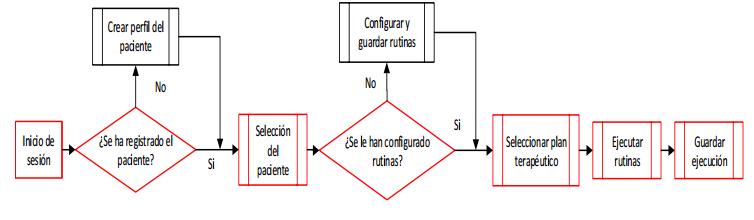
\includegraphics[scale=0.3]{images/diagram-therapy.png}
        \caption{Secuencia principal para la realización de la terapia asistida con el uso de la aplicación}
        \label{fig: diagram-therapy}
    \end{figure}

    
    \subsubthesischapter{Panel de configuración de las rutinas}
\end{thesischapter}